\documentclass{beamer}
\usetheme{Boadilla}

\usepackage{minted}
\usepackage{hyperref}
\usepackage{datetime}
\usepackage{datenumber}
\usepackage{advdate}
\usepackage[super]{nth}
\usepackage{hyperref}
\usepackage{graphicx}
\usepackage{caption}
\usepackage{subcaption}
\graphicspath{ {./images/} }

\parindent 0pt \parskip 6pt

\newcommand\todo[1]{\textbf{TODO(ag939): #1}}
\newcommand\haskell[1]{\mintinline{haskell}{#1}}
\newcommand\monospace[1]{\mintinline{text}{#1}}


\title[Thesis Presentation]{Measuring Mutual Information inside Deep Neural Networks}
\author{\texorpdfstring{Andrius Grabauskas - ag939}{Andrius Grabauskas
}}


\begin{document}

	\frame {
		\titlepage
	}
	\frame {
		\frametitle{Quick recap:}
		\begin{itemize}

			\item{
          We do not actually understand or know why DNN`s learn.
      } \item {
          N. Tishby suggested that DNN`s learn as a result of compression
          between the layers and the information bottleneck principle.
          \footnote{\url{https://arxiv.org/abs/1703.00810}}

      } \item {
          N. Tishby`s claims have been disputed by A. M. Saxe who claimed that
          his results are due to the parameters he chose.
          \footnote{\url{https://openreview.net/forum?id=ry\_WPG-A-}}
      } \item {
          I am here to:
          \begin{itemize}
            \item Reproduce Tishby`s results provided in his paper.
            \item Explore new ways to verify Tishby`s core thesis.
            \item Provide stable code that could be extended and used by other
              in the future.
          \end{itemize}
      }
		\end{itemize}
	}	
  \frame {
    \frametitle{Success criteria}
    \begin{itemize}
      \item Reproduce results in Tishby`s paper
      \item {
          Essentially reproduce this image and show that the results are stable
          with varying parameters.
          \begin{figure}
            \centering
            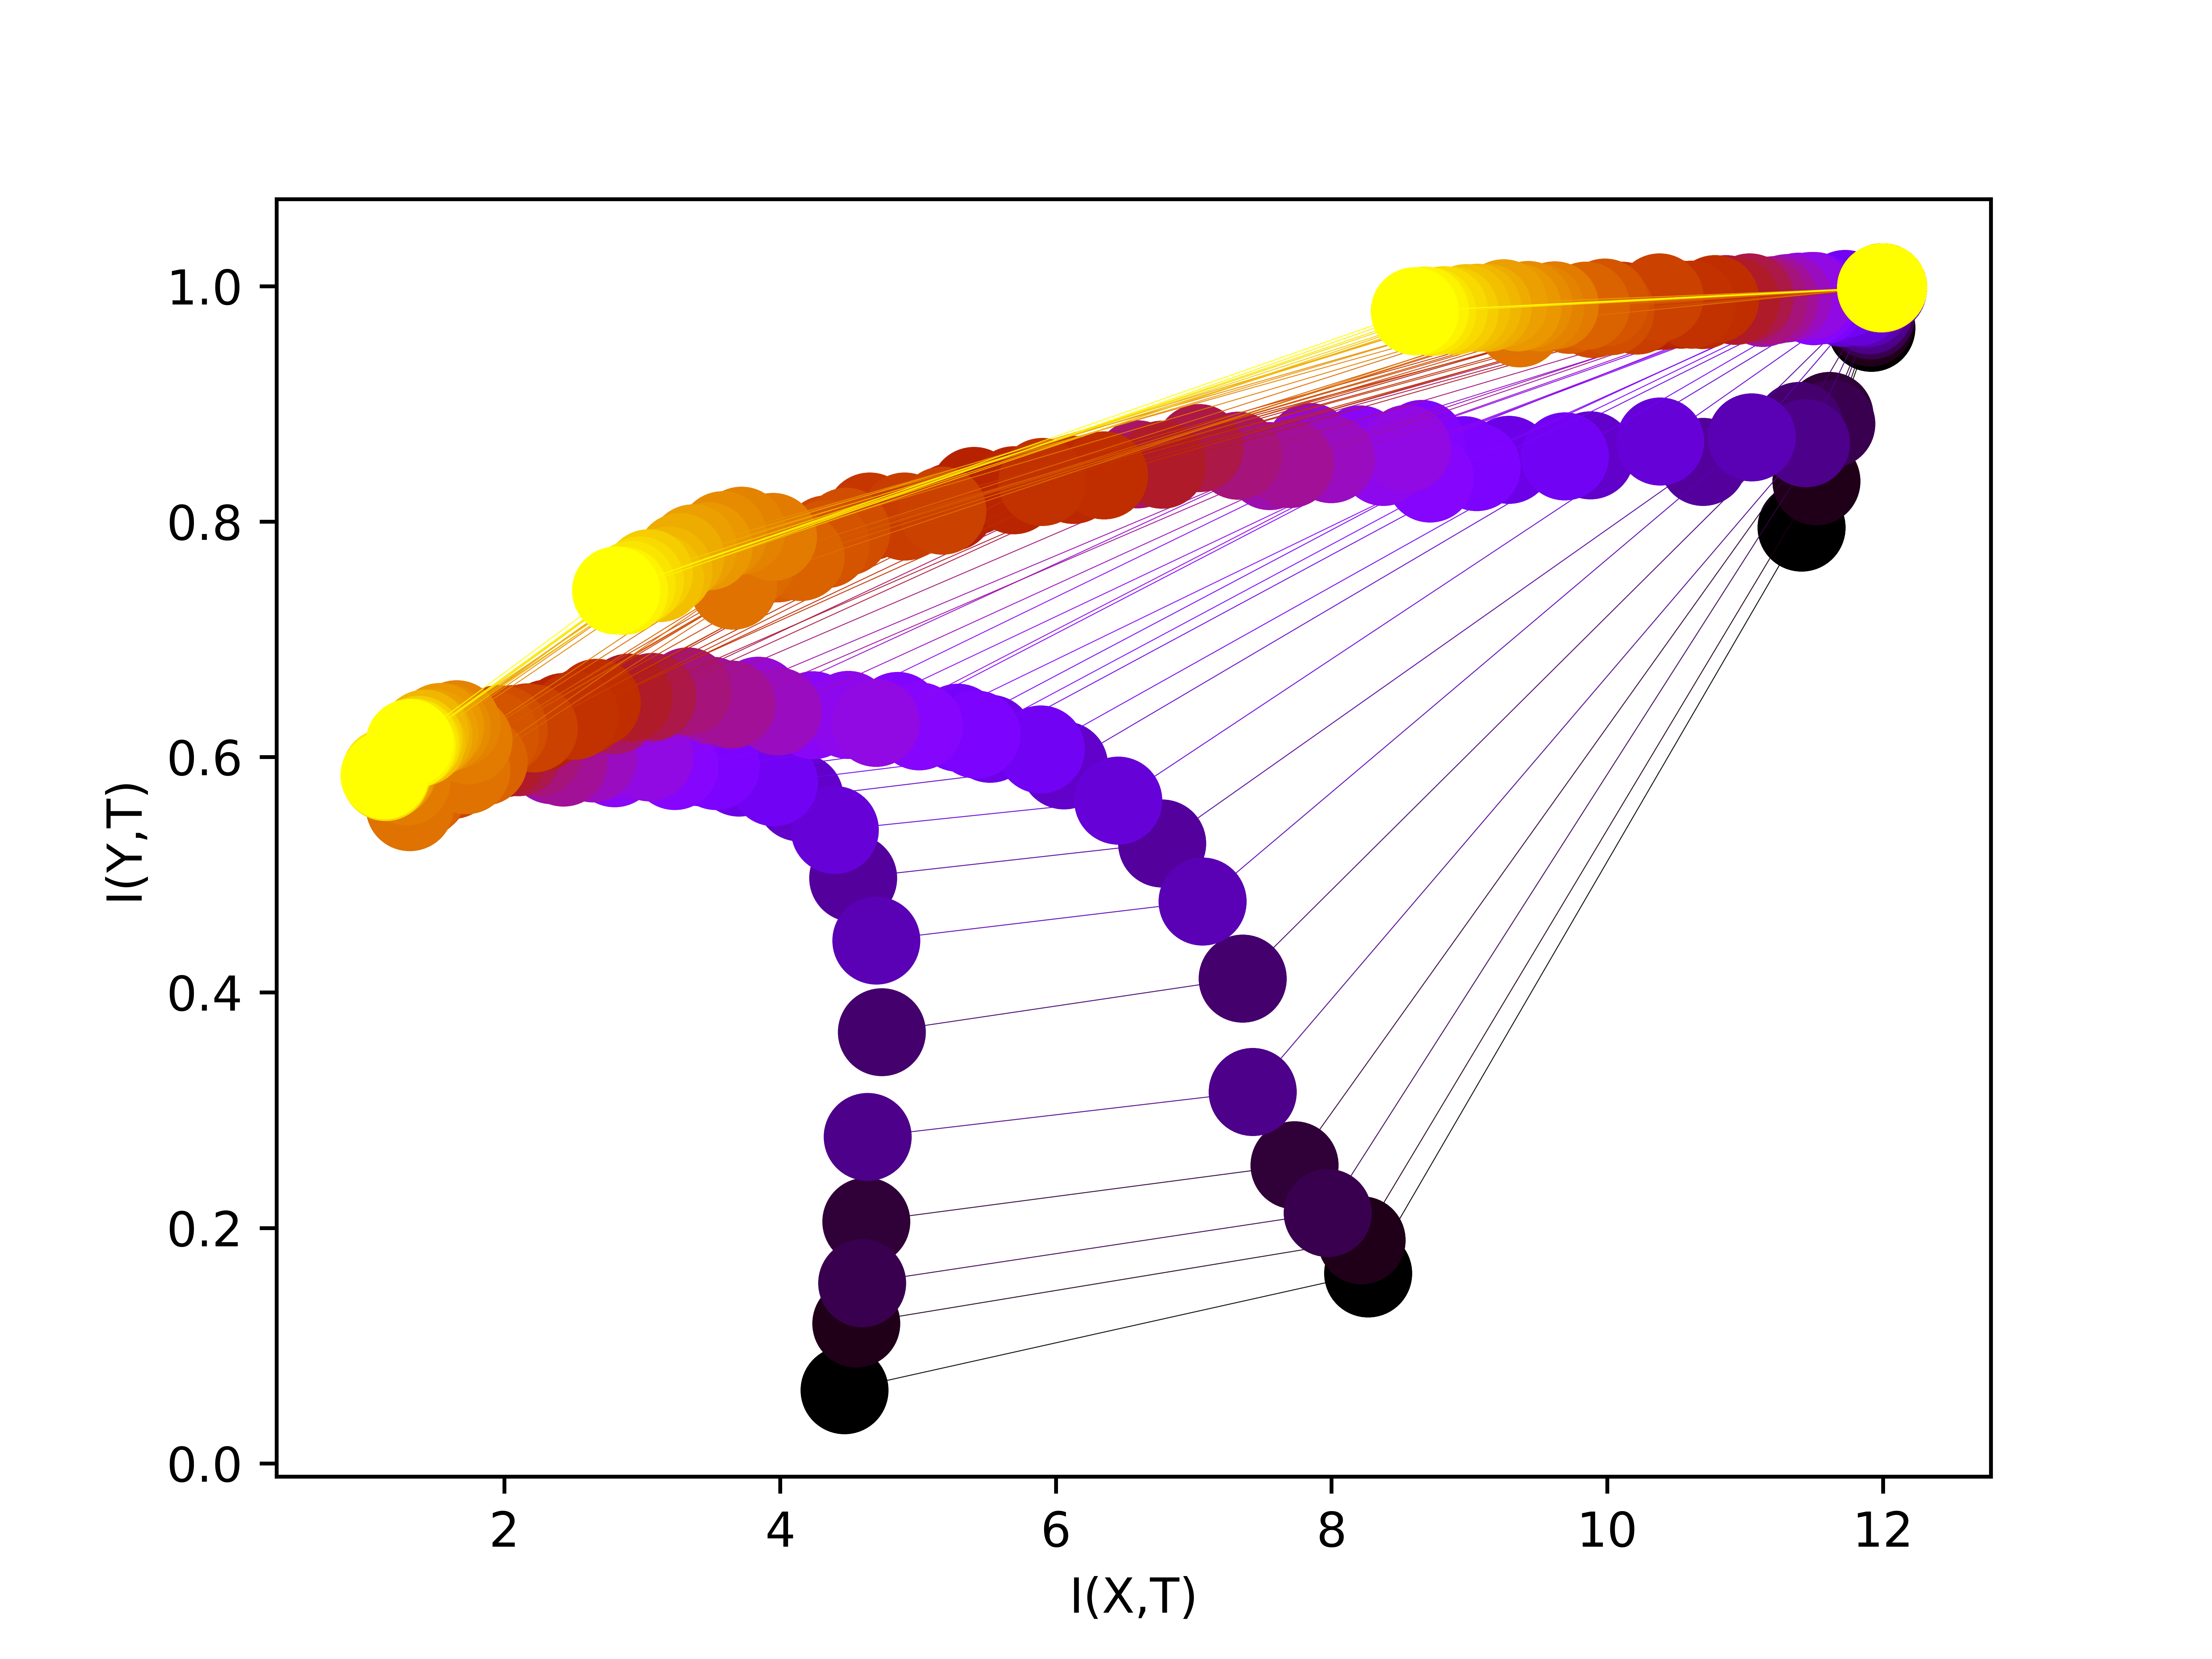
\includegraphics[height=0.65\textheight, width=\textwidth,
            keepaspectratio=true]{a.png}
          \end{figure}
      }
    \end{itemize}


  }
  \begin{frame}[plain, noframenumbering]
    \begin{figure}
      \centering
      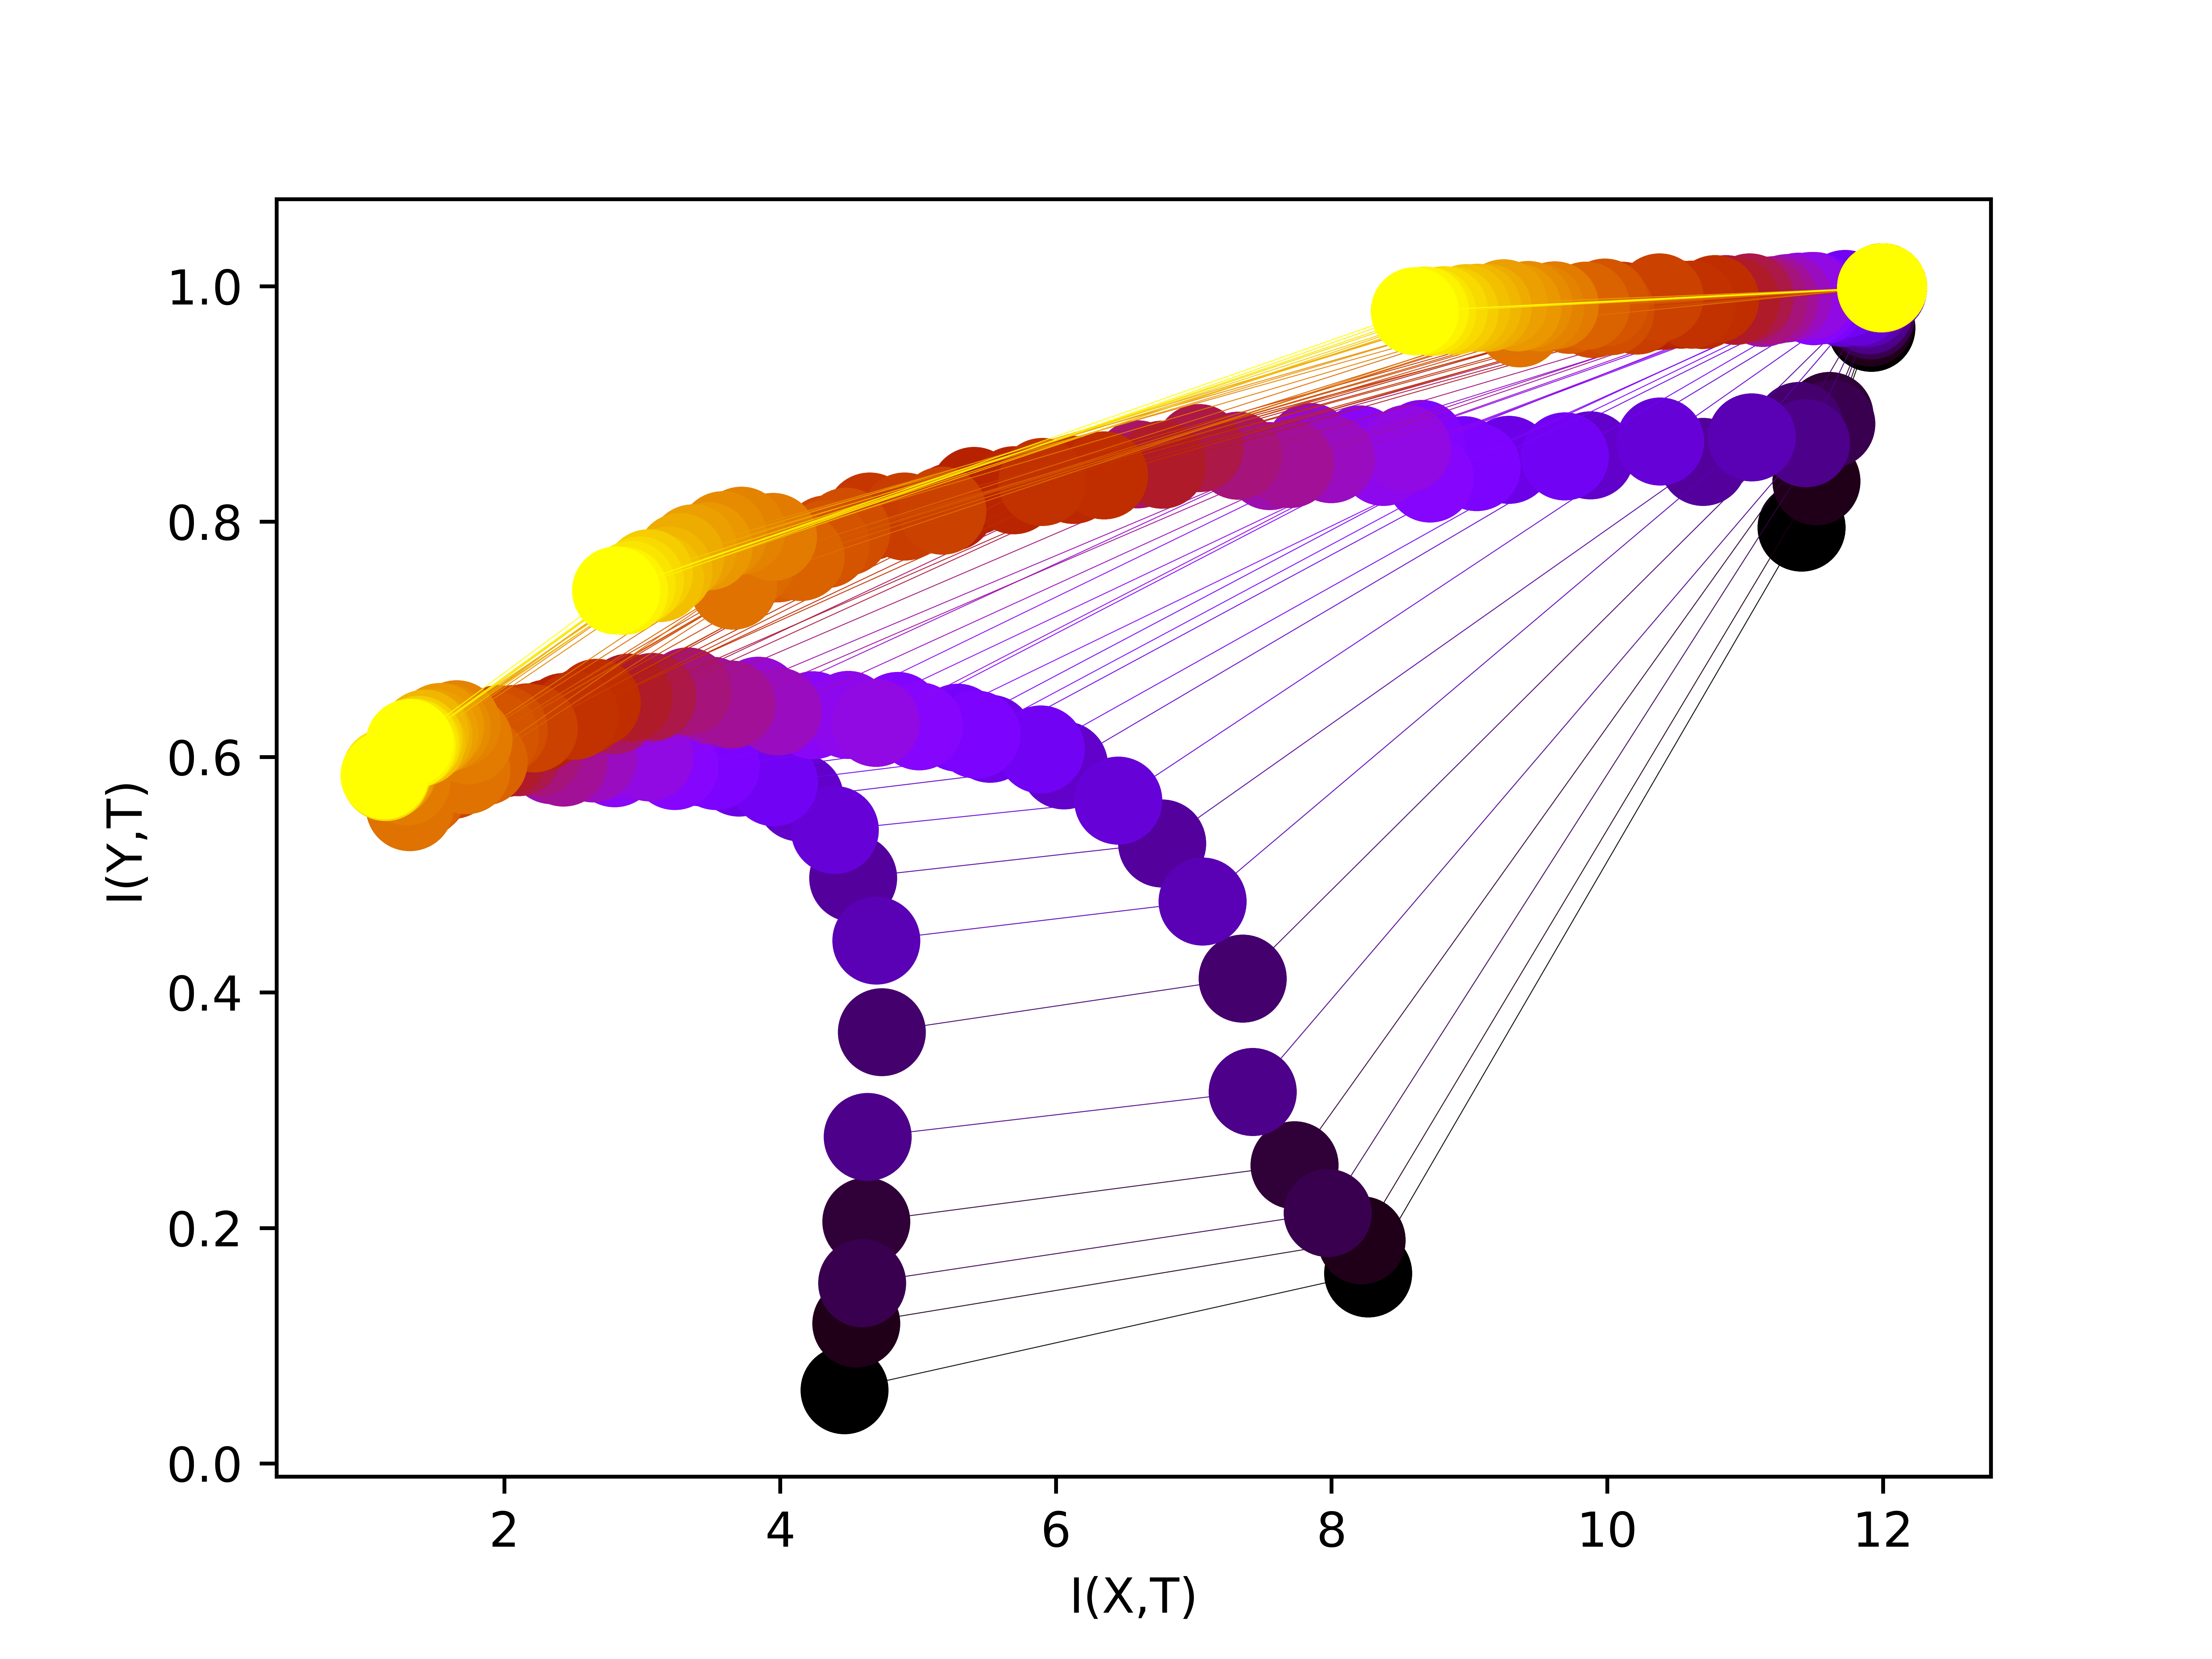
\includegraphics[height=\textheight, width=\textwidth,
      keepaspectratio=false]{a.png}
    \end{figure}
  \end{frame}
  \addtocounter{page}{-2}
  \frame {
    \frametitle{Current progress}

    \begin{itemize}
      \item{
          Reimplemented Tishby`s code and reproduced his results.
      }
      \item {
          Found evidence that Tishby`s Mutual Information Estimator (MIE) might
          not be completely sound.
      }
      \item {
          Had lots of trouble with finding an alternative MIE as Neural Networks
          are have high dimensionality which doesn't play well with some MIE.
      }
      \item {
          Settled with Kernel Density Mutual (KDE) MIE, which agreed with
          Tishby`s results. (Although it is by far not a perfect measure of
          information)
      }

    \end{itemize}
  }
  \frame {
    \frametitle{Remaining work, Issues}
      \begin{itemize}
        \item{ 
          Show that the results hold for a bigger dataset such as MNIST
        }
        \item{ 
          Clean up and comment the code such that it is easy to understand and
          extensible by others.
        }
        \item{ 
          At the core of Tishby`s thesis is the notion that Weights of a NN are
          random
          \begin{itemize}
            \item{
                What does it actually mean for a weight of a NN to be random ?
            } 
            \item {
                given that at every point in time a weight is fixed and non
                changing.
            }
          \end{itemize}
        }
      \end{itemize}
  }

\end{document}
